\section{Fonctionnement}

\subsection{Interface}

Notre génération de ville se présente par une interface dans laquelle il est possible d'opter pour deux options :
		- générer une ville aléatoirement 
		- paramétrer la ville que l'on veut générer

\begin{center}
	\centering
    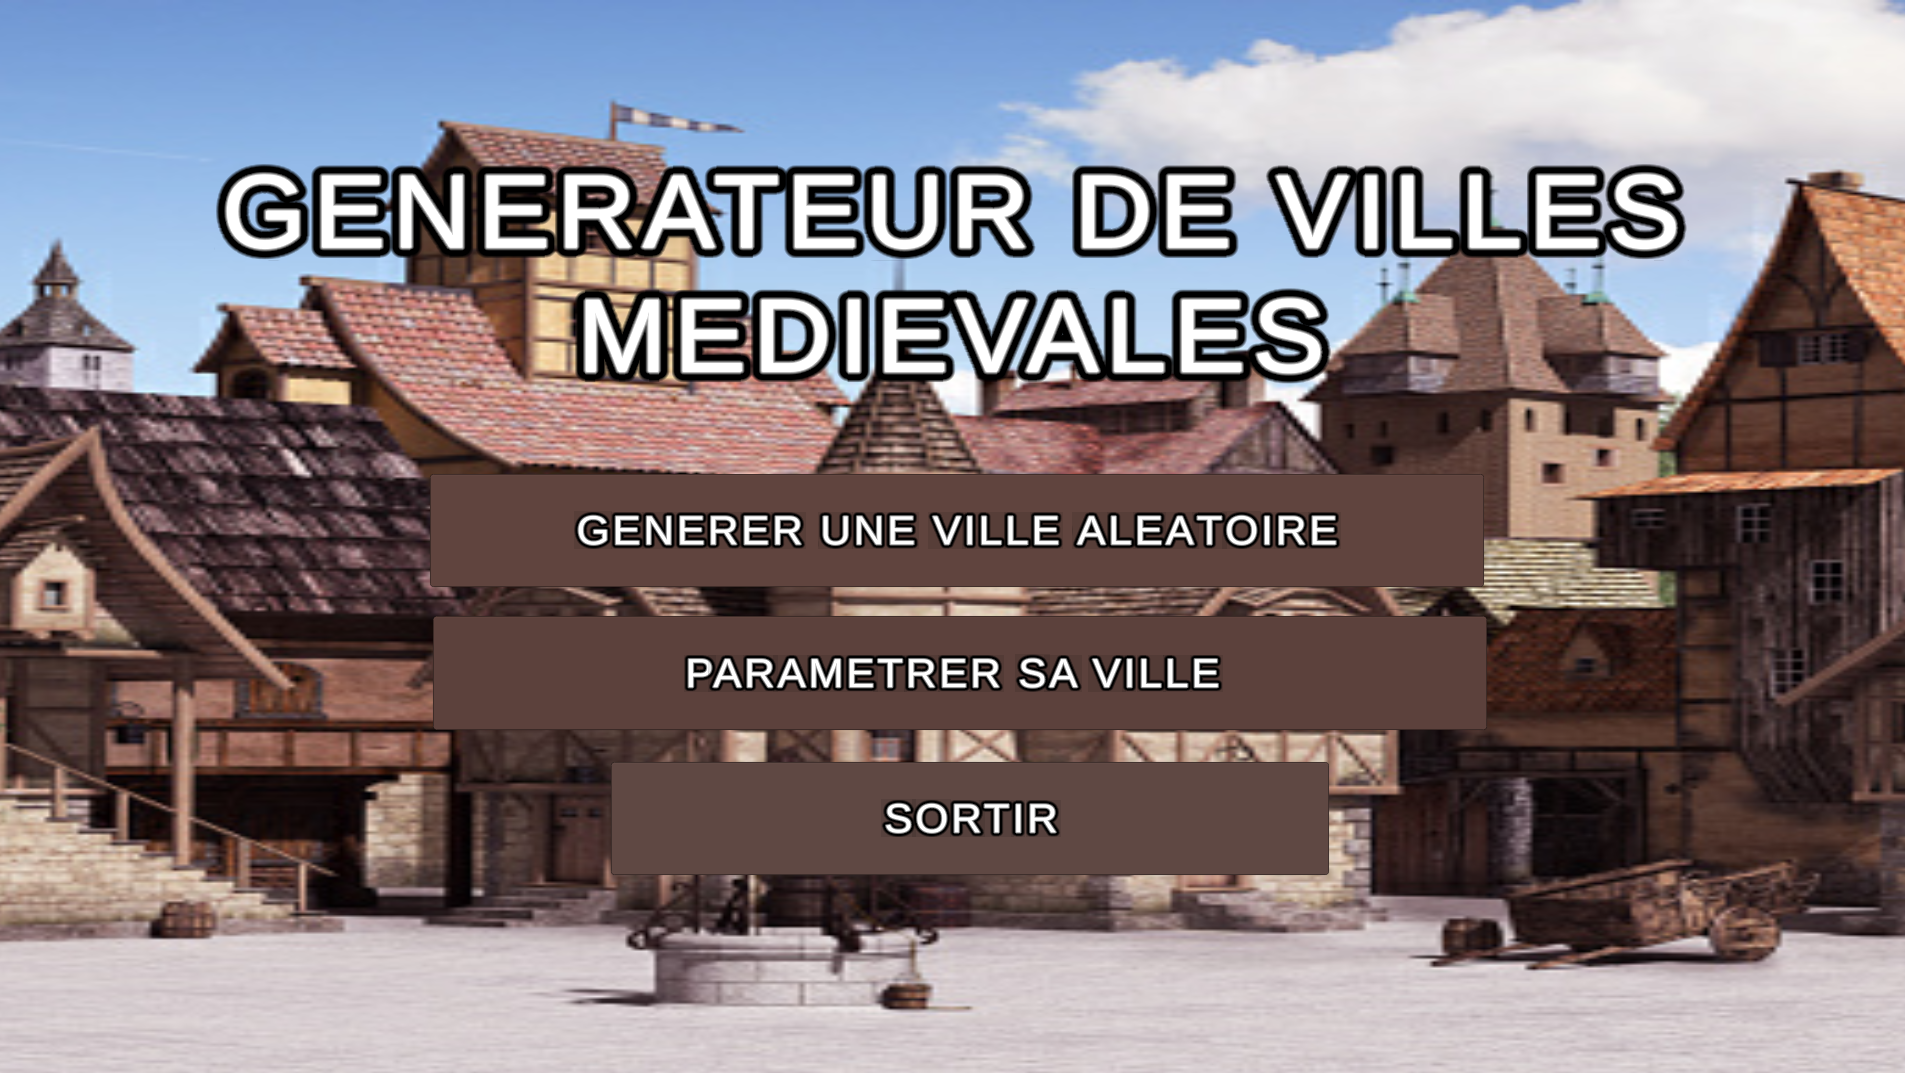
\includegraphics[height = 5 cm]{images/Interface_1.png}\\
\end{center}

Lorsque l'on décide de paramétrer la ville que l'on veut générer on a alors trois nouvelles options possibles :
\begin{itemize}
	\item gérer le type du terrain sous forme de curseur qui plus la jauge est à gauche plus le terrain est plat, plus elle est a droite plus le terrain va être en relief avec des chaînes montagneuses.
	\item gérer la taille du terrain sous forme de curseur aussi qui en fonction de  la taille choisie va influencer le nombre de routes, de bâtiments, et la taille de la muraille.
	\item décider si l'on veut une rivière sur le plan de la ville ou non.
\end{itemize}

\begin{center}
	\centering
    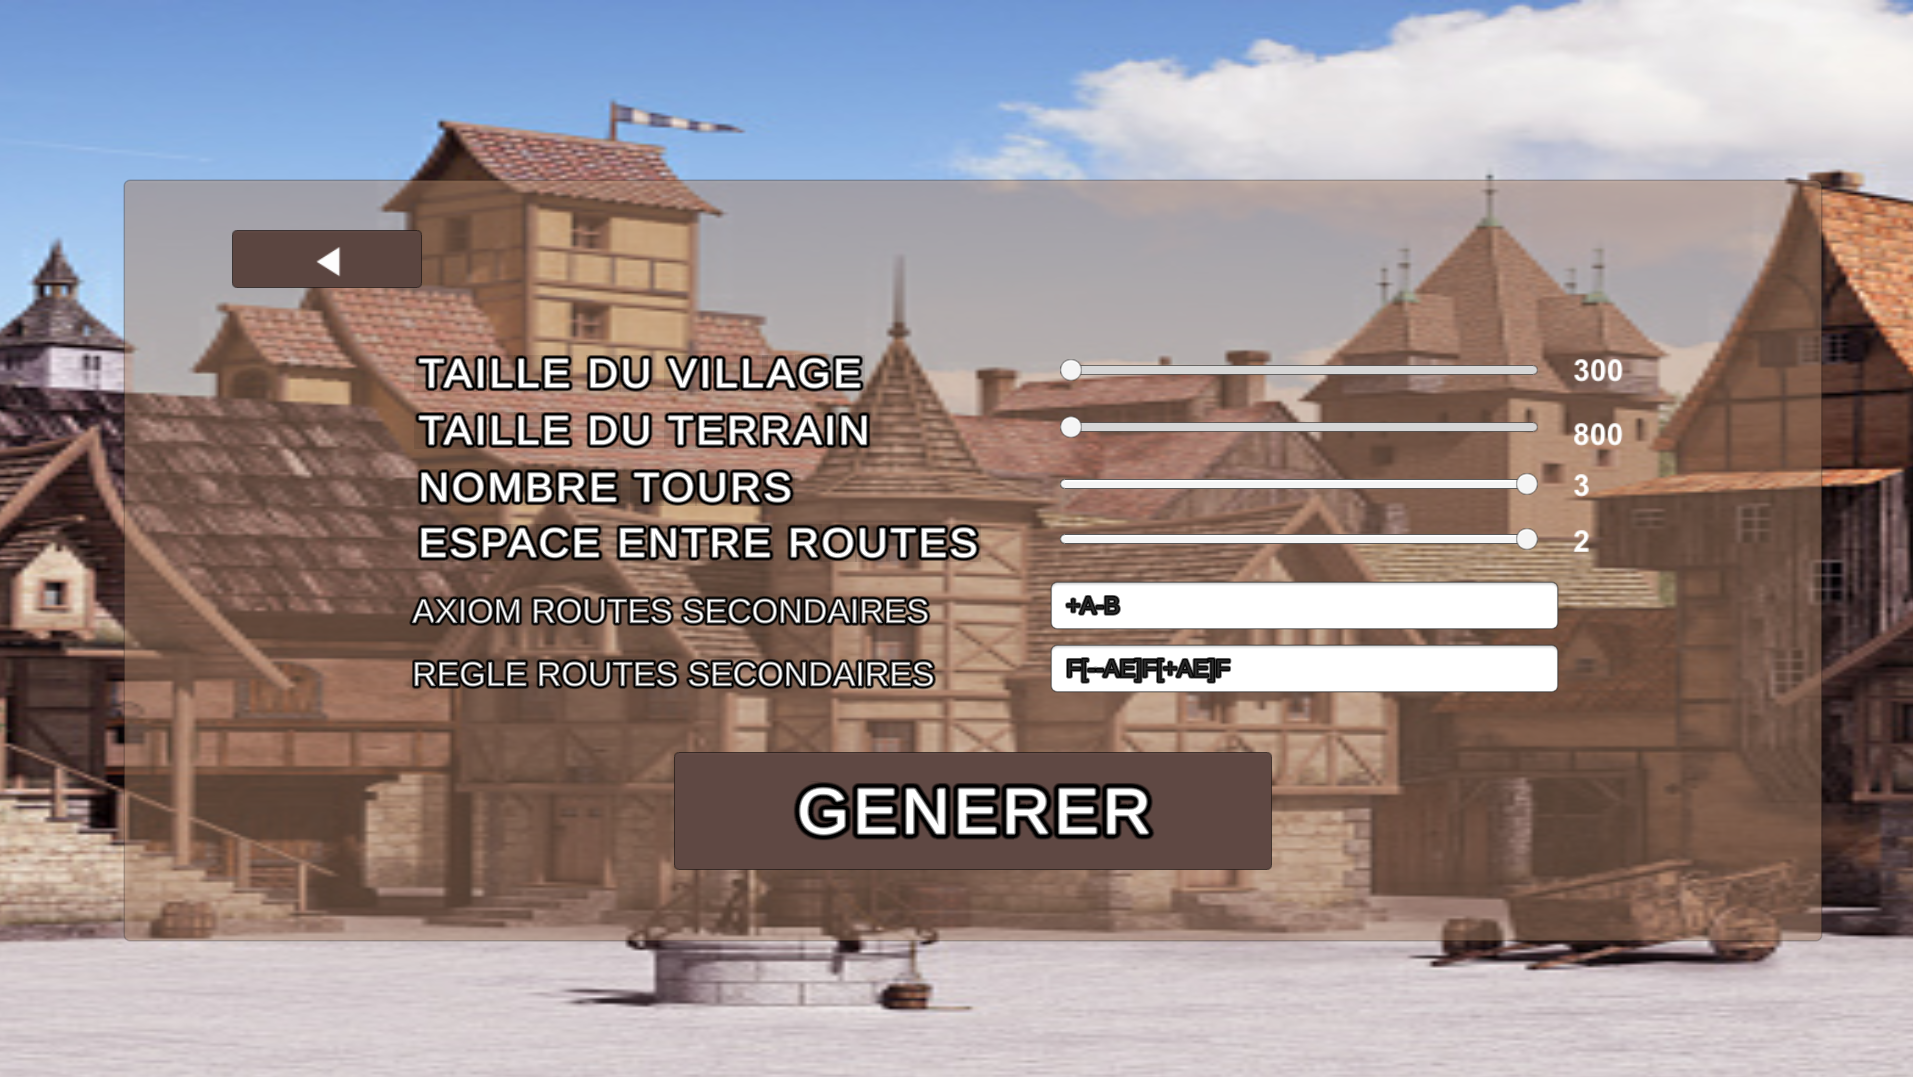
\includegraphics[height = 5 cm]{images/Interface_2.png}\\
\end{center}

En fonction des paramètres choisis, une ville sera alors générée aléatoirement et représentera un certain nombre de bâtiments placés dans des cellules avec des routes secondaires et principales apparentes, avec des éléments environnementaux comme des arbres ou des éléments un peu plus décoratifs comme des fontaines, des lampadaires ou des charettes pour rappeler le côté médiéval.

\begin{center}
	\centering
    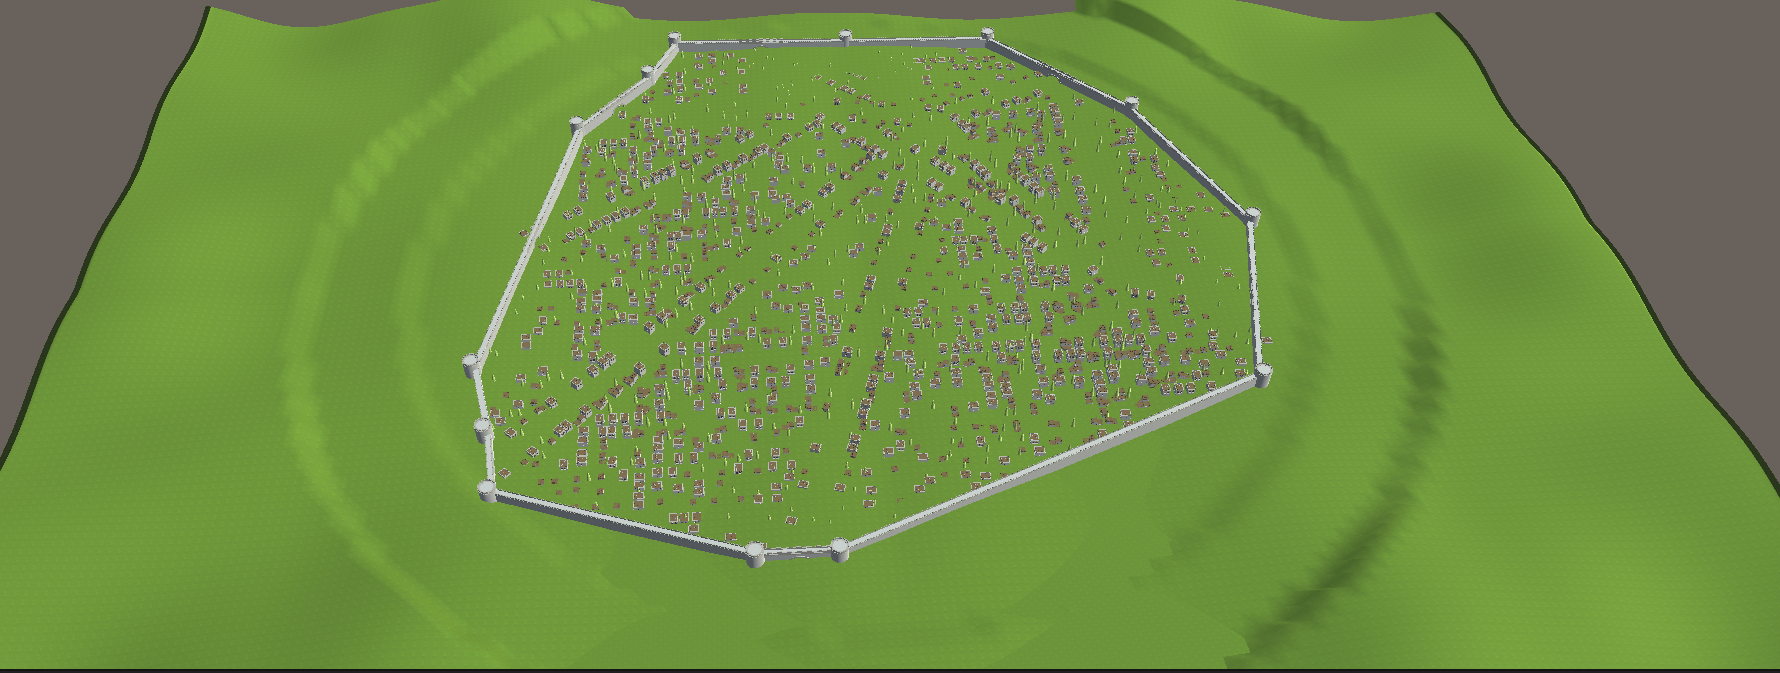
\includegraphics[height = 5 cm]{images/Ville_1.png}\\
\end{center}

La ville sera alors entourée d'une muraille pour délimiter son expansion et permettre aussi de rendre plus plat le terrain sur lequel est placé cette muraille pour ne pas avoir de contraintes de placement de ce,lule en relief à l'intérieur de la muraille.

\begin{center}
	\centering
    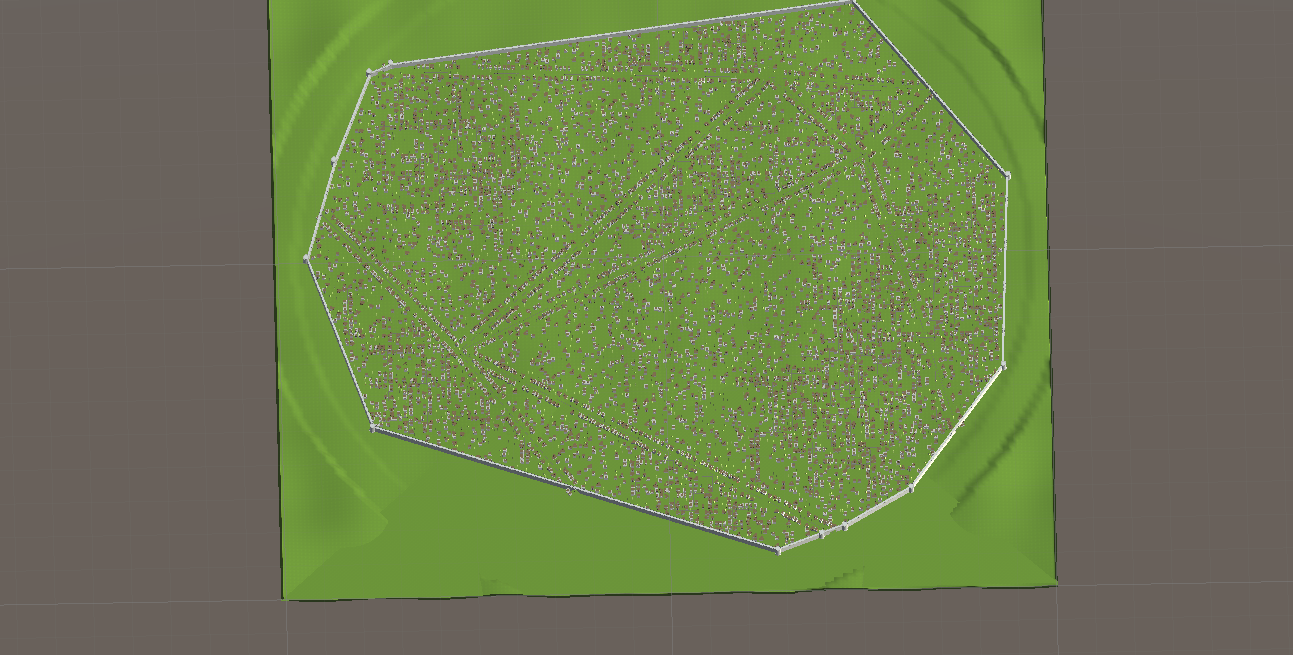
\includegraphics[height = 5 cm]{images/Ville_2.png}\\
\end{center}

L’interface a été faite avec l’outil UI sur une scène, et est donc composée de scripts en C Sharp permettant l’exécution d’une action suite à une interaction avec les différents éléments de l’interface. Lorsque l'on clique sur un bouton, c'est l'appel à la fonction C Sharp qui permet l'affichage de l'éxecution du code voulu. Les scènes en question sont numérotées et mises en place dans les paramètres de Build, ce qui permet l'affichage d'une scène de l'interface et une scène de génération de ville. 

\subsection{Génération de terrain}

La génération de terrain se fait par l'algorithme de Perlin, en théorie lorsqu'on sélectionne "Générer une ville " on affiche un terrain en relief créé par le bruit de Perlin, dans lequel la surface où se situe la ville est plane, et le contour de celle-ci est en relief, on a également des creux autour des montagnes qui représente les points d'eaux mis en place (rivières). Le relief peut être plus ou moins prononcé en fonction des coordonnées que l'on veut établir au code, plus les coordonnées seront élevées plus le bruit de Perlin sera prononcé et donc on aura un terrain avec des hautes montagnes et quasiment aucun endroit où la surface est plane (hors la ville car le code applatit la zone où on la place).

\begin{center}
	\centering
    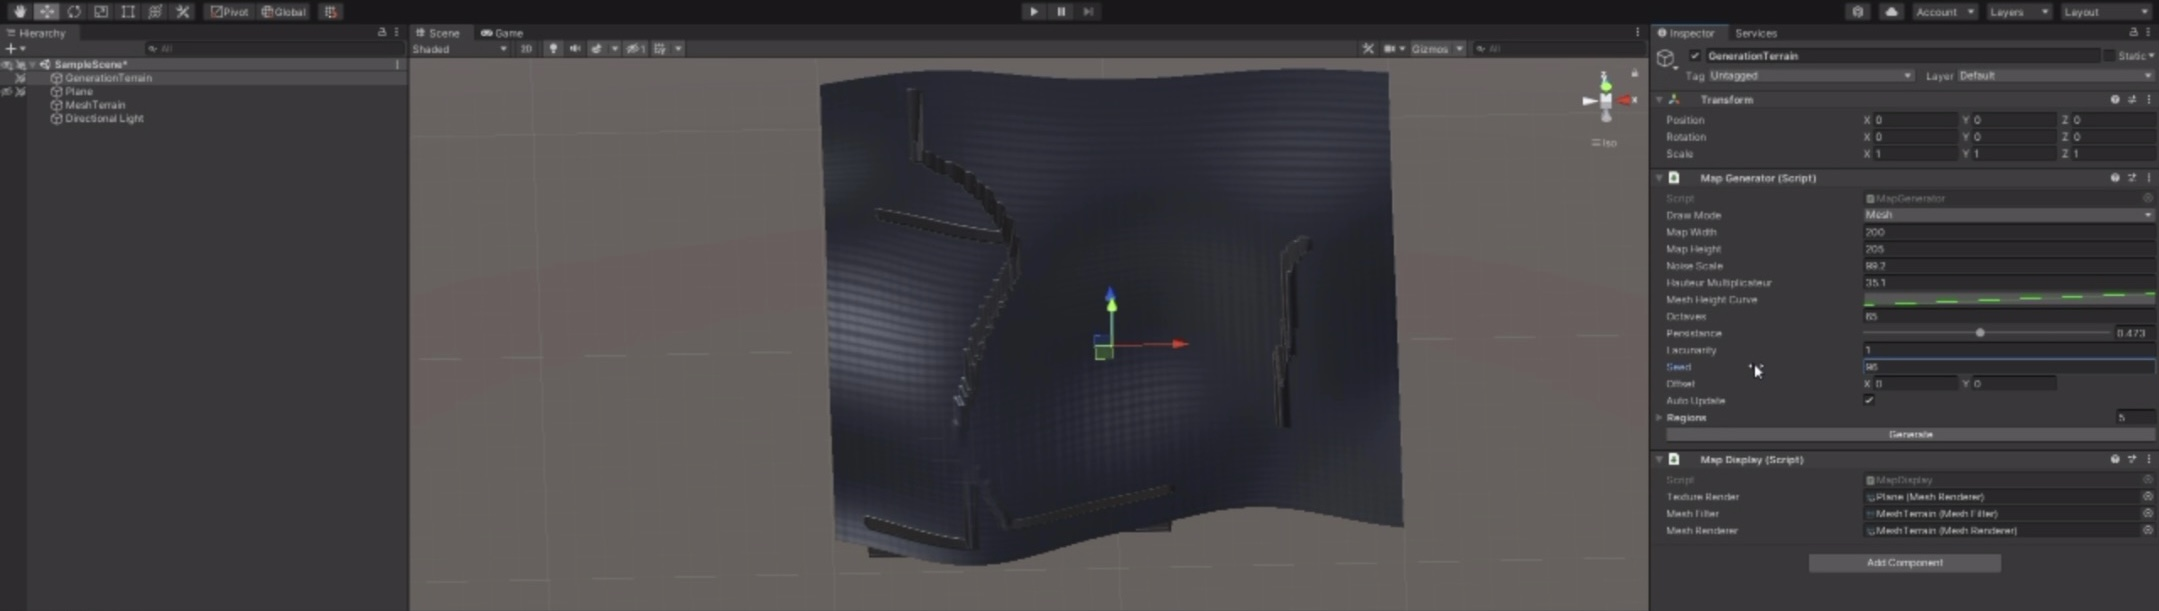
\includegraphics[height = 5 cm]{images/terrainavecriviere.jpeg}\\
\end{center}

\subsection{Génération de la ville}

La génération de la ville est aléatoire, on obtient un certain nombre de bâtiments à l'intérieur de la muraille, les bâtiments sont le plus possible placés à proximité des routes pour éviter d'avoir une génération trop aléatoire et une ville qui se rapproche le plus d'une ville urbaine, dans lequel on y retrouve des quartiers entourés par des routes secondaires, et un alignement de bâtiments autour des routes principales. Les routes sortent de la ville par des portes créées à l'intérieur de la muraille. On observe également des bâtiments à l'exterieur de la muraille mais on y reviendra dans la section bugs.

\begin{center}
	\centering
    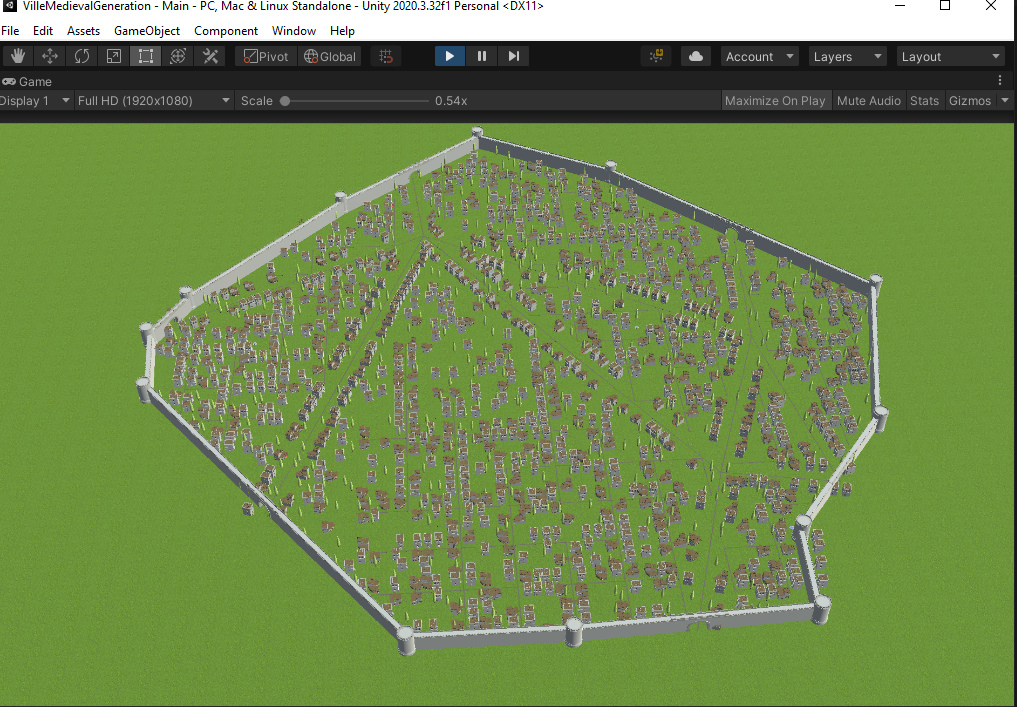
\includegraphics[height = 5 cm]{images/generationville.png}\\
\end{center}





